\section{Results: heat and the irrigated--rainfed maize gap}
\label{sec:maize}

This section reports the main result, then the checks that shape how far it can be trusted. All tests are those fixed in the specification unless stated otherwise.

\subsection{The data at a glance}

In the main sample (\MaizeMainDeps{} departments, \MaizeMainPairs{} department-years), irrigated grain maize yields \YieldIrr{} quintals per hectare on average, against \YieldRain{} for rainfed maize. The median gap is \GapMedianPct\,\%, and the irrigated yield is above the rainfed one in all but \GapNotAboveCount{} of the \MaizeMainPairs{} department-years (it is lower in \GapBelowCount). The question is not whether irrigated maize yields more, but how this advantage moves with summer heat.

\subsection{Main result}
\label{subsec:maize-main}

\Cref{tab:maize-hyp} reports the main hypothesis, its replication and the four secondary hypotheses.

\begin{table}[H]
\centering
\small
\caption{Maize: main and secondary hypotheses (July--August, maize mask)}
\label{tab:maize-hyp}
\begin{threeparttable}
{\setlength{\tabcolsep}{3.5pt}% GÉNÉRÉ par scripts/26_tables_memoire.py (phase4bis_q1_hypotheses.csv)
\begin{tabular}{>{\raggedright}p{4.6cm}rrrrrrr}
\toprule
Hypothesis & Estimate & \% per DD & \shortstack{$p$ boot.\\one-sided} & \shortstack{$p$\\Holm} & \shortstack{$p$ clust.\\dept.} & $n$ & Years \\
\midrule
H1: gap, heat ($\beta > 0$) & $+0.0158$ & $+1.59$ & 0.007 & --- & 0.009 & 435 & 2000--2025 \\
Replication 2000--2009: gap, heat & $+0.0108$ & $+1.09$ & 0.049 & --- & 0.196 & 165 & 2000--2009 \\
H2a: gap, soil moisture ($\delta < 0$) & $-0.3517$ &  & 0.012 & 0.024 & <0.001 & 435 & 2000--2025 \\
H2b: rainfed yield, heat ($< 0$) & $-0.0256$ & $-2.52$ & <0.001 & <0.001 & 0.001 & 435 & 2000--2025 \\
H2c: irrigated yield, heat ($< 0$) & $-0.0098$ & $-0.97$ & 0.002 & 0.005 & <0.001 & 435 & 2000--2025 \\
H3: gap, heat $\times$ crisis days ($< 0$) & $+0.0008$ &  & 0.961 & 0.961 & 0.005 & 168 & 2016--2025 \\
\bottomrule
\end{tabular}
}
\begin{tablenotes}\footnotesize
\item ``\% per DD'': $100\,(e^{\hat\beta}-1)$, change per degree-day above 32\,$^{\circ}$C. ``$p$ boot.'': restricted wild cluster bootstrap by year, 9,999 draws, in the direction of the hypothesis; the only inference used for conclusions. ``$p$ Holm'': corrected over the family H2a--H3. ``$p$ clust.\ dept.'': two-sided, clustered by department, shown for information only (its size is wrong, \cref{sec:inference}). The size of the bootstrap was measured for H1 and, afterwards, for the replication (\ReplSize\,\% with 10 clusters, \cref{subsec:maize-repl}) and for H2b and H2c (\HtwobSize\,\% and \HtwocSize\,\%); it was not measured for H2a, nor for H3, which also rests on 10 clusters.
\end{tablenotes}
\end{threeparttable}
\end{table}

\paragraph{H1 is established under the pre-specified rule.} Each degree-day above 32\,$^{\circ}$C in July--August is associated with a \QonePct\,\% wider yield gap in favour of irrigated maize ($p = \QoneP$). The measured size of this test on the same data is \QoneSizeWCR\,\%, below the 10\,\% limit. ``Established'' is meant in the sense of this rule only. \ExploPairs{} of the \MaizeMainPairs{} department-years (\ExploSharePct\,\%) belong to 2010--2025, the period whose exploratory analysis suggested the hypothesis; the only new evidence is the decade 2000--2009, examined next. A diagnostic added after publication of the first version, declared in the log before it was computed (\cref{app:deviations}), measures the power of this test with the same placebo: it detects a true effect of the estimated size (0.016) in \PowerFull\,\% of cases and half of it in \PowerHalf\,\% (size under the null in this run: \PowerCheckSize\,\%).

\paragraph{The result does not rest on the SAFRAN temperature analysis.} A second check added after the first version recomputes the July--August degree-days from E-OBS, a gridded data set interpolated from station records \parencite{cornes2018}, with the same double-sine method, window and maize mask. It was declared in the log, with its reading rule, before it was computed, but the log was not committed beforehand (\cref{app:deviations}). The two measures are correlated at \EobsCorr. With E-OBS heat, the estimate is \EobsPct\,\% per degree-day, with a one-sided $p = \EobsP$, so under the declared rule H1 does not depend on the temperature source. E-OBS counts more degree-days above 32\,$^{\circ}$C than SIM in these departments, so coefficients per degree-day are not directly comparable: one within-department standard deviation of heat is associated with a gap wider by \EobsSdEffect\,\% with E-OBS and \SimSdEffect\,\% with SIM. The check is partial: part of the French stations behind E-OBS also feed SAFRAN, only the main model was re-estimated, and the soil wetness control still comes from SIM.

\paragraph{Checks added after a simulated review.} Four more analyses were declared in the log before being computed, after a simulated peer review of the first version (\cref{app:deviations}); the log was not committed beforehand. (i) Inverting the bootstrap gives a 90\,\% interval for $\beta$ of \CiNinetyLow{} to \CiNinetyHigh\,\% per degree-day (95\,\%: \CiNinetyFiveLow{} to \CiNinetyFiveHigh\,\%). The sign is supported; the magnitude is known only to within a factor of eight. (ii) Without the soil wetness index, the estimate is \NoSwiPct\,\% ($p = \NoSwiP$); with the July--August climatic water balance (precipitation minus evapotranspiration) in its place, \PetPct\,\% ($p = \PetP$). Under the declared rule, the association does not depend on the moisture control chosen, but heat and drought remain mixed: within departments, degree-days above 32\,$^{\circ}$C and the water balance are correlated at $\CorrPet$. (iii) Departments: see \cref{subsec:maize-measure}. (iv) Decades: see the replication below.

\paragraph{Both modes lose, rainfed maize much more.} Each degree-day is associated with about \QoneRainfedPct\,\% lower rainfed yields and about \QoneIrrigatedPct\,\% lower irrigated yields; both are significant after the Holm correction, and the size of these two tests, measured afterwards with the same placebo as H1, is \HtwobSize\,\% and \HtwocSize\,\%. Rainfed maize is about \QoneRatio{} times more sensitive to heat. Irrigation is therefore associated with a smaller sensitivity, not with its disappearance. Wetter soils are associated with a narrower gap ($\hat\delta = \QoneSwi$ per unit of the soil wetness index), as expected if the advantage of irrigated maize comes from water.

\paragraph{Water restrictions (H3).} The slope of the gap on heat is not smaller where crisis-level water restrictions lasted longer; the interaction even has the opposite sign ($p_{\text{Holm}} = \QoneHthreeP$). This result is not interpretable causally. Restrictions are decided during the driest summers and in the driest departments, so their duration is tied to the very conditions that drive the gap. Which mechanism produces the positive interaction is a question I did not test. Possible ones, none checked: restrictions are decided where the gap is already widening; the indicator counts days with at least one zone of the department at crisis level, which does not say whether irrigated maize was restricted; and orders may exempt some uses. The indicator is also coarse, and the sample has only 10 summers. For water policy, this is the most directly relevant result of the monograph, and it does not show that restrictions reduced the advantage of irrigated maize.

\subsection{Replication on years never used}
\label{subsec:maize-repl}

The exploratory analysis that motivated this question had used 2010--2025. On 2000--2009 alone, a decade that no earlier analysis had touched, the estimate keeps its sign: \QoneReplPct\,\% per degree-day, with a one-sided $p = \QoneReplP$. The same mask gives \QoneRecentPct\,\% on 2010--2025, so the estimate for the earlier decade is about half as large. On 2000--2009 without 2003, the point estimate is larger than on 2010--2025 (\cref{tab:maize-measure}): the smaller estimate over the decade comes from 2003, which raises a question about linearity, taken up below.

Three cautions apply. The two-sided $p$-value is \QoneReplPtwo; the test rests on 10 years: measured afterwards with the same placebo, the size of the bootstrap with 10 clusters is \ReplSize\,\%, but its power against a true effect of the estimated size is only \ReplPower\,\%, so a $p$-value near 0.05 is weak evidence; and, as shown below, the replication holds with the maize mask but not with department-wide weather. Moreover, in the weighted model 2003 alone carries \LevThreeEarly\,\% of the residual variation of heat over 2000--2009 ($N_{\mathrm{eff}} = \NeffLevEarly$, against \LevThree\,\% and \NeffLevAll{} over 2000--2025; \cref{subsec:maize-v12}): the replication is essentially a test on one summer. I read it as consistent in sign, not as a confirmation of magnitude. An interaction between heat and the decade 2000--2009, added after the review, finds no detectable difference between the two slopes ($\DecDiff$, two-sided $p = \DecDiffP$; without 2003, $\DecDiffNoThree$, $p = \DecDiffNoThreeP$): the data cannot say whether the earlier decade is really less sensitive.

\subsection{Robustness}

\Cref{tab:maize-rob} and \cref{fig:maize-rob} report the pre-specified robustness checks and the one added later, declared before it was estimated.

\begin{table}[H]
\centering
\small
\caption{Maize: robustness of the main estimate}
\label{tab:maize-rob}
% GÉNÉRÉ par scripts/26_tables_memoire.py (phase4bis_q1_robustesse.csv, phase4bis_q1_r9_masque2008.csv)
\begin{tabular}{lrrrrr}
\toprule
Specification & $\hat\beta$ & \% per DD & $p$ boot.\ one-sided & $n$ & Depts \\
\midrule
Main specification & $+0.0158$ & $+1.59$ & 0.007 & 435 & 17 \\
38 departments (all quality statuses) & $+0.0217$ & $+2.19$ & 0.006 & 981 & 38 \\
2010--2025 only & $+0.0242$ & $+2.45$ & 0.030 & 270 & 17 \\
Weather weighted by department area & $+0.0104$ & $+1.05$ & 0.221 & 435 & 17 \\
Threshold 30\,$^{\circ}$C & $+0.0104$ & $+1.05$ & 0.007 & 435 & 17 \\
July only & $+0.0575$ & $+5.92$ & 0.013 & 435 & 17 \\
Unweighted & $+0.0185$ & $+1.86$ & 0.021 & 435 & 17 \\
Without 2025 (provisional) & $+0.0157$ & $+1.59$ & 0.015 & 418 & 17 \\
Without 2003 & $+0.0243$ & $+2.46$ & 0.029 & 418 & 17 \\
2008 maize mask (added later) & $+0.0153$ & $+1.54$ & 0.007 & 435 & 17 \\
\bottomrule
\end{tabular}

\end{table}

\begin{figure}[H]
\centering
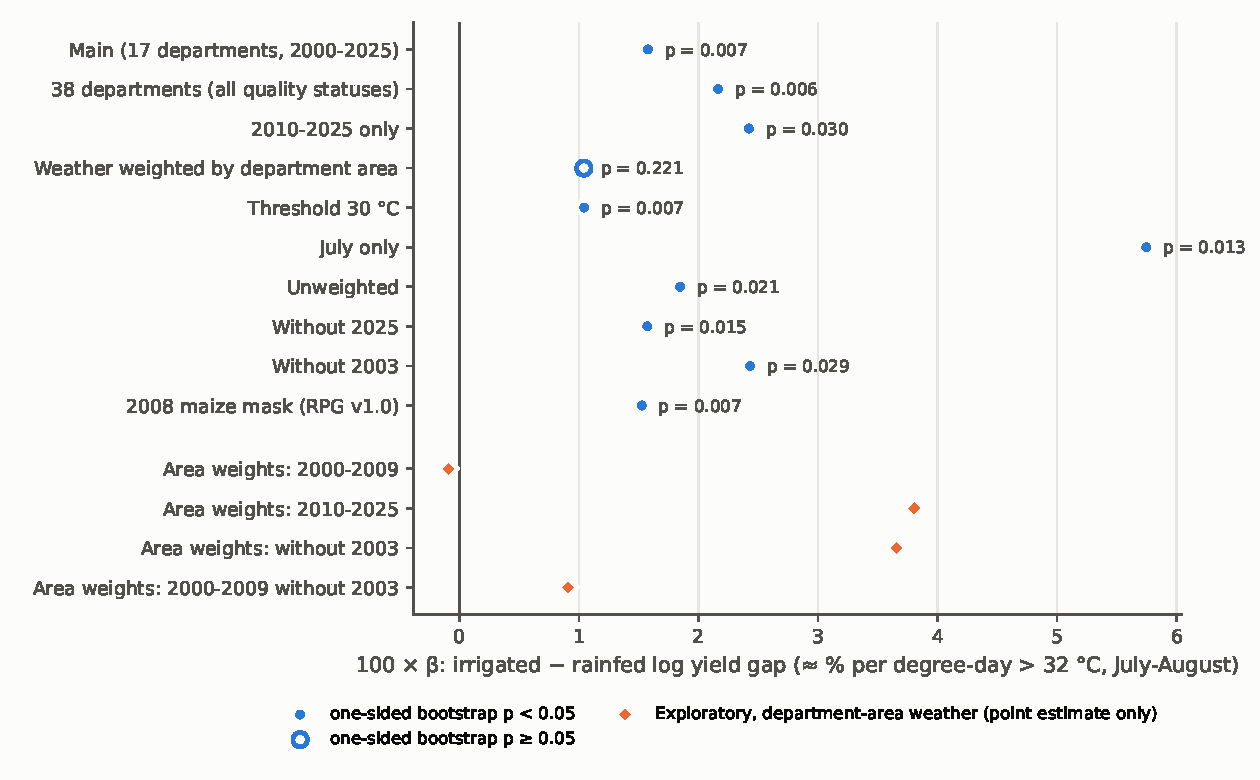
\includegraphics[width=0.95\textwidth]{figures/fig4_mais_robustesse.pdf}
\caption{Coefficient of the main model by specification. Circles: pre-specified and added checks, with the one-sided bootstrap $p$-value; open circle: $p \ge 0.05$. Diamonds: exploratory point estimates with department-area weather, by period, without inference. No intervals are drawn: an interval obtained by inverting the bootstrap was computed for the main specification only (\CiNinetyLow{} to \CiNinetyHigh\,\% at 90\,\%, \cref{subsec:maize-main}), and intervals clustered by year have not had their size checked.}
\label{fig:maize-rob}
\end{figure}

The sign is positive in all \QoneRobN{} specifications and significant in \QoneRobSig. The estimate holds without 2003, the dominant summer; without the provisional year 2025; in the \MaizeDeps{} departments of all quality statuses (\QoneAllDepsPct\,\%); with a 30\,$^{\circ}$C threshold; with July alone; and without weights. With a maize mask drawn from 2008 parcel blocks (grain and silage maize), about eight years older, it is unchanged (\QoneMaskPct\,\%, $p = \QoneMaskP$). One check fails: with weather weighted by the department's surface, the estimate falls to \QoneAreaPct\,\% and is not significant ($p = \QoneAreaP$).

\subsection{Does the result depend on how heat is measured?}
\label{subsec:maize-measure}

Yes, and this is the main limitation of the result. \Cref{tab:maize-measure} shows where the two measures diverge.

\begin{table}[H]
\centering
\small
\caption{Maize: coefficient by heat measure and period (point estimates, exploratory, no inference)}
\label{tab:maize-measure}
% GÉNÉRÉ par scripts/26_tables_memoire.py (phase4bis_q1_exploratoire.csv)
\begin{tabular}{lrr}
\toprule
Period & Maize mask & Department area \\
\midrule
2000--2025 & $+0.0158$ & $+0.0104$ \\
2000--2009 & $+0.0108$ & $-0.0009$ \\
2010--2025 & $+0.0242$ & $+0.0381$ \\
Without 2003 & $+0.0243$ & $+0.0365$ \\
2000--2009 without 2003 & $+0.0380$ & $+0.0091$ \\
\bottomrule
\end{tabular}

\end{table}

The divergence is concentrated in 2000--2009 ($\MaskEarly$ with the maize mask, $\AreaEarly$ with department area) and persists in that decade even without 2003. On 2010--2025, department-wide weather gives a \emph{larger} coefficient (\AreaRecent{} against \MaskRecent).

What we know about the two measures is the following.
\begin{itemize}
  \item \textbf{The age of the mask is not the cause.} A mask drawn from 2008 blocks gives almost the same exposure as the 2015--2017 mask and the same estimate.
  \item \textbf{The department-area measure understates the 2003 heat where maize grows in departments with uplands.} In \ReliefCount{} such departments, maize fields lie \ReliefAltDiffMin{} to \ReliefAltDiffMax{}~m below the department's average altitude, and department-wide weather understates their 2003 heat by up to \ReliefGapMax{} degree-days (\cref{tab:relief}). This is shown for 2003 only, while the divergence persists on 2000--2009 without 2003. An error that scaled heat by the same factor every year would rescale $\beta$, not remove it; removing the association requires errors that reorder departments from one year to the next, which is not shown.
  \item \textbf{Neither measure is checked against where each mode grows.} Both masks assign the same heat to irrigated and rainfed maize. In departments with uplands, irrigated maize may sit lower in the valleys than rainfed maize, so the mask may describe the heat of irrigated fields better than that of rainfed ones.
  \item \textbf{The maize mask was the measure designated in advance} as the main one, before any estimate on 2000--2009 was computed.
  \item \textbf{The choice did not favour the result already known.} When the specification was written, the only known estimate (phase 6, 2010--2025) used department-wide weather and was significant. On those same years the maize mask gives a smaller estimate (\MaskRecent{} against \AreaRecent).
\end{itemize}
These points favour the maize mask. They do not explain the whole divergence, nor why department-wide weather gives a stronger association over 2010--2025, and the altitude pattern was sought after the results were known. Two checks added after the review settle part of this. Dropping one department at a time leaves the estimate between \LooMinPct{} and \LooMaxPct\,\% per degree-day, significant in \LooSig{} cases out of 17. Dropping the six departments with uplands together gives \NoReliefPct\,\% with $p = \NoReliefP$ on the remaining 11: under the rule declared before this check, H1 depends on these departments. Without them the estimate is smaller and less precise; a later check finds no detectable difference between the slopes of the two groups (interaction $+\RelInter$, two-sided $p = \RelInterP$; \cref{subsec:maize-v12}), so the loss of significance is consistent with the remaining 11 departments simply carrying less information. Either way, the significance of the result comes from the very departments where the choice of heat measure matters, which is consistent with the altitude pattern but also means that the measure and the sample cannot be separated. The honest summary is that the result holds when heat is measured where maize is grown, and that it is sensitive to that choice in the earlier decade and rests on the departments with uplands.

\subsection{Is the composition of land moving with heat?}

If hot years changed which land is irrigated, the gap could move for reasons unrelated to irrigation itself. A descriptive check, not pre-specified, is whether the irrigated share of grain maize area moves with heat. With the same fixed effects and controls, one more degree-day above 32\,$^{\circ}$C is associated with a change of $\CompEst$ in the irrigated share ($p = \CompP$, clustered by year, for information only). This check has little power by construction. Areas are largely decided at sowing, before the summer heat, so it cannot detect the more plausible threat: rainfed maize sown for grain but harvested as silage in dry summers, which the yield data do not show; a later descriptive check with the SAA areas of silage maize, available for 2010--2025, finds no detectable increase in the share of rainfed maize harvested as silage in hotter summers (one-sided $p = \SilageP$, mean share \SilageShare\,\%; \cref{subsec:maize-v12}), but this check misses 2003 and silage areas may be recorded before harvest; abandoned fields stay in the statistics with a zero yield. The absence of a detected response is not evidence that composition is stable.

\subsection{What it is worth}

\Cref{tab:valuation} turns the main estimate into quantities for three hot summers. For each department, the extra production associated with irrigation \emph{in a summer hotter than the department's normal} is
\[
\text{irrigated area} \times \text{rainfed yield} \times \big[e^{\hat\beta\,(\ddthirtytwo - \text{department mean})} - 1\big],
\]
valued at the maize price of the year in current euros. Applying the factor to the rainfed yield is the cautious choice; applied to the irrigated yield, the 2003 figure would be about \ValAltPct\,\% higher. The formula extrapolates the linear estimate to 2003, far above the other summers. It also applies to each summer's whole excess heat, national part included, a slope that is identified from differences between departments within a year; in the regression, the national part of each summer is absorbed by the year effects. A simple check suggests it overstates the 2003 figure by about \ValOverPct\,\%: in 2003, the observed gap exceeded each department's average gap by \GapObsTwoThousandThree{} in log terms on average, against \GapPredTwoThousandThree{} predicted by $\hat\beta$.

\begin{table}[H]
\centering
\small
\caption{Production associated with irrigation in hot summers (17 departments, descriptive)}
\label{tab:valuation}
\begin{threeparttable}
{\setlength{\tabcolsep}{4pt}% GÉNÉRÉ par scripts/26_tables_memoire.py (phase4bis_q1_valorisation.csv)
\begin{tabular}{lrrrrrr}
\toprule
Summer & \shortstack{Heat vs.\\normal (DD)} & \shortstack{Irrigated\\area (kha)} & \shortstack{Quintals\\(millions)} & \shortstack{Price\\(EUR/q)} & \shortstack{Value\\(M EUR)} & \shortstack{90\,\% range\\(M EUR)} \\
\midrule
2003 & $+$13.7 & 213 & 2.98 & 16.4 & 49 & 8--98 \\
2019 & $+$2.5 & 195 & 0.43 & 21.3 & 9 & 2--17 \\
2022 & $+$1.9 & 161 & 0.33 & 41.3 & 14 & 3--25 \\
\bottomrule
\end{tabular}
}
\begin{tablenotes}\footnotesize
\item ``Heat vs.\ normal'': area-weighted mean excess of $\mathrm{DD}_{>32}$ over each department's 2000--2025 mean. The range recomputes the value at the bounds of the 90\,\% interval of $\hat\beta$ obtained by inverting the bootstrap by year; it is wide and asymmetric because the bounds enter an exponential. Prices: INSEE index scaled to Eurostat absolute prices over 2012--2016.
\end{tablenotes}
\end{threeparttable}
\end{table}

In the 17 departments, the extra production associated with irrigation in the summer of 2003 is worth about \QoneValTwoThousandThree{} million euros (indicative range \QoneValLow{} to \QoneValHigh). In 2022, fewer quintals are worth more than in 2019 because the price of maize was about twice as high. These figures are gross production values in current euros. They are not the total value of irrigation, which also includes its average advantage; not a value net of the cost of water, energy and labour; not a value per cubic metre or the cost of a water restriction; and not a causal gain. They also leave out the part of the advantage associated with drier soils, since $\beta$ is measured at a given soil wetness.

\subsection{Further checks requested after the audit}
\label{subsec:maize-v12}

A third batch of analyses was declared in the log before being computed, after an internal audit of this text; the log was not committed beforehand, none was pre-specified, and none changes the status of H1. \Cref{tab:maize-v12} summarises them.

\begin{table}[htbp]
\centering
\caption{Maize: further checks (exploratory, declared before computation)}
\label{tab:maize-v12}
\small
\begin{tabular}{p{7.3cm}p{6.2cm}}
\toprule
Check & Result \\
\midrule
\multicolumn{2}{l}{\textit{Inference on H1 ($\hat\beta = \QoneBeta$; bootstrap by year: $p = \QoneP$)}} \\
Cluster jackknife by year (CV3), $t$ with 25 d.f. & one-sided $p = \CvThreeP$ \\
Randomisation inference, 5,000 derangements of years & one-sided $p = \RiP$ \\
Double machine learning (random forests on SWI, P, ETP, growing degree-days; folds by blocks of years) & $\hat\beta = \DmlBeta$, one-sided $p = \DmlP$ \\
\midrule
\multicolumn{2}{l}{\textit{Size of the bootstrap test (300 placebos, nominal 5\,\%)}} \\
H1, heat permuted across departments within each year & \WithinYearSize\,\% \\
H2b (rainfed) and H2c (irrigated), years permuted & \HtwobSize\,\% and \HtwocSize\,\% \\
Placebo Conley matrices corrected by \texttt{fixest} & \ConleyFixedPct\,\% of repetitions \\
\midrule
\multicolumn{2}{l}{\textit{Heterogeneity of the slope}} \\
Heat $\times$ uplands (six departments) & $+\RelInter$, two-sided $p = \RelInterP$ \\
Heat $\times$ irrigated share of grain maize & two-sided $p = \IrrInterP$ \\
Department slopes, empirical Bayes shrinkage & $\tau = \EbTau$, homogeneity $p = \EbQp$; shrunk slopes \EbMin{} to \EbMax \\
Causal forest, calibration test of heterogeneity & $p = \ForestP$ \\
\midrule
\multicolumn{2}{l}{\textit{Other}} \\
Share of rainfed maize harvested as silage, 2010--2025 & no increase with heat, one-sided $p = \SilageP$ \\
Wind capacity and yields \parencite[cf.][]{kaffine2019} & one $p < 0.05$, negative (irrigated yield), not robust to Holm \\
\bottomrule
\end{tabular}
\end{table}

\paragraph{Inference.} The rule of phase 4 bis rests on the bootstrap by year, and it is unchanged. Two other valid procedures do not agree on the strength of the evidence. Randomisation over permuted years gives a smaller $p$-value, but its null leaves the true effect of heat in the error, as the placebo does. The cluster jackknife, which \textcite{mackinnon2023} recommend when clusters are few and unequal in leverage, gives $p = \CvThreeP$: with it, H1 would not be significant at 5\,\%. This is consistent with the concentration of leverage on 2003 (\LevThree\,\% of the weighted residual variation of heat, $N_{\mathrm{eff}} = \NeffLevAll$). The partially linear model of \textcite{chernozhukov2018}, with flexible weather controls, leaves $\hat\beta$ almost unchanged. The new placebo suggested by the review, which keeps each summer's heat in its own year and shuffles it across departments, gives a size of \WithinYearSize\,\%, within the limit of the rule.

\paragraph{Heterogeneity.} None of the three approaches finds a detectable difference in the slope between departments: not by uplands, not by the irrigated share of maize, not by the shrinkage estimator, whose departmental slopes all lie between \EbMin{} and \EbMax{} (they correlate at $\EbCorIrr$ with the irrigated share and $+\EbCorAlt$ with the altitude gap, on 17 points). A causal forest \parencite{athey2019} is uninformative with 435 observations: its calibration test detects no heterogeneity and its average effect is very imprecise. With 17 departments, the data cannot say where the association is stronger.

\paragraph{Variables that were not kept.} The wind capacity installed in each department, built from the national register of electricity installations, is not associated with yields in the way reported for the United States by \textcite{kaffine2019}; the register only lists installations in service in 2026, and departments are too coarse for a local microclimate effect. A satellite measure of surface temperature, which would capture the cooling of irrigated fields \parencite{zhu2022,siebert2017}, was declared but not computed, for lack of access to the NASA service at the time of writing.

\subsection{Summary}

In the main sample, summer heat is associated with a wider yield advantage of irrigated over rainfed maize. The association satisfies the rule fixed before any estimation on 2000--2009, although \ExploSharePct\,\% of its sample comes from the years that suggested it; keeps its sign, with weak evidence, on a decade the exploratory analysis had not used; and survives an older parcel mask and another temperature source. Its magnitude is uncertain and rests largely on 2003; it is not significant without the six departments with uplands (although the slope does not differ detectably between the two groups) or with a cluster jackknife ($p = \CvThreeP$). It depends on measuring heat where maize is grown, a choice made in advance and supported by the geography of the departments concerned, but one that matters. It is an association, not the causal effect of irrigation.
